\chapter{Arus Listrik dan Efeknya}\label{ch:g8:electric-current-effects}

Arusnya sudah berarak tanpa nama namun berguna sepanjang lima tahun
rangkaian: menyalakan benang, memutar \omterm{ex:g6:circuits-and-safety:motor}{motor}, membunyikan bel. Tahun
ini kelistrikan berubah menjadi kuantitatif --- alat ukur, \omterm{def:g6:measurement-in-science:measuring}{satuan}, dan
hukum --- dan kita membuka dengan menghitung persediaan: apa,
tepatnya, yang dapat \emph{dilakukan} sebuah arus? Ternyata ada tiga
efek, dan seluruh dunia kelistrikan dibangun darinya.

\section{Ketiga efeknya}

\begin{proposition}[Efek arus listrik]\label{prop:g8:electric-current-effects:three}
Arus yang mengalir menembus materi memperlihatkan dirinya lewat tiga
efek:
\begin{enumerate}
  \item \emph{efek panas}\index{efek panas}: setiap arus
        menghangatkan penghantar yang diseberanginya --- dengan lembut
        pada kawat yang baik, dengan garang pada kawat yang tipis atau
        kelebihan beban, sampai berpijar putih dengan sengaja pada
        filamen dan pemanggang roti;
  \item \emph{efek magnet}\index{efek magnet}: sebuah arus mengubah
        sekelilingnya menjadi bersifat \omterm{def:g1:magnets:magnet}{magnet} --- sepotong kawat
        menyimpangkan jarum \omterm{def:g4:magnets-and-compass:compass}{kompas} di dekatnya, dan kawat yang
        digulung menjadi \omterm{def:g1:magnets:magnet}{magnet} sejati berkutub, yang dapat
        dinyalakan sesuka hati;
  \item \emph{efek kimia}\index{efek kimia}: ketika menyeberangi
        \omterm{def:g3:solids-liquids-gases:liquid}{zat cair} tertentu, sebuah arus menggerakkan perubahan kimia
        --- memecah air menjadi dua \omterm{def:g3:solids-liquids-gases:gas}{gas}, menyepuh sendok dengan
        perak, serta mengisi dan mengosongkan setiap \omterm{def:g3:first-electric-circuit:battery}{baterai}.
\end{enumerate}
\end{proposition}

\begin{example}[Efek panas sedang bekerja]\label{ex:g8:electric-current-effects:heating}
Yang disengaja: batang pemanggang roti yang berpijar, kumparan
tersembunyi di dalam cerek, filamen lampu lama yang berpijar putih,
\omterm{def:g7:short-circuits-safety:fuse}{sekring} yang dibangun untuk melebur paling dahulu. Yang tidak
diinginkan: pengisi daya telepon yang hangat, bagian bawah komputer
jinjing yang panas --- dan ancaman \omterm{def:g7:short-circuits-safety:device}{korsleting}, yang kamu pelajari
sebagai tanda tangan sang penjahat. Satu efek, pelayan sekaligus
bahaya, yang takarannya ditentukan oleh seberapa keras arusnya
berlari --- takaran yang kita pelajari untuk \emph{diukur} pada bab
berikutnya.
\end{example}

\begin{omfigure}
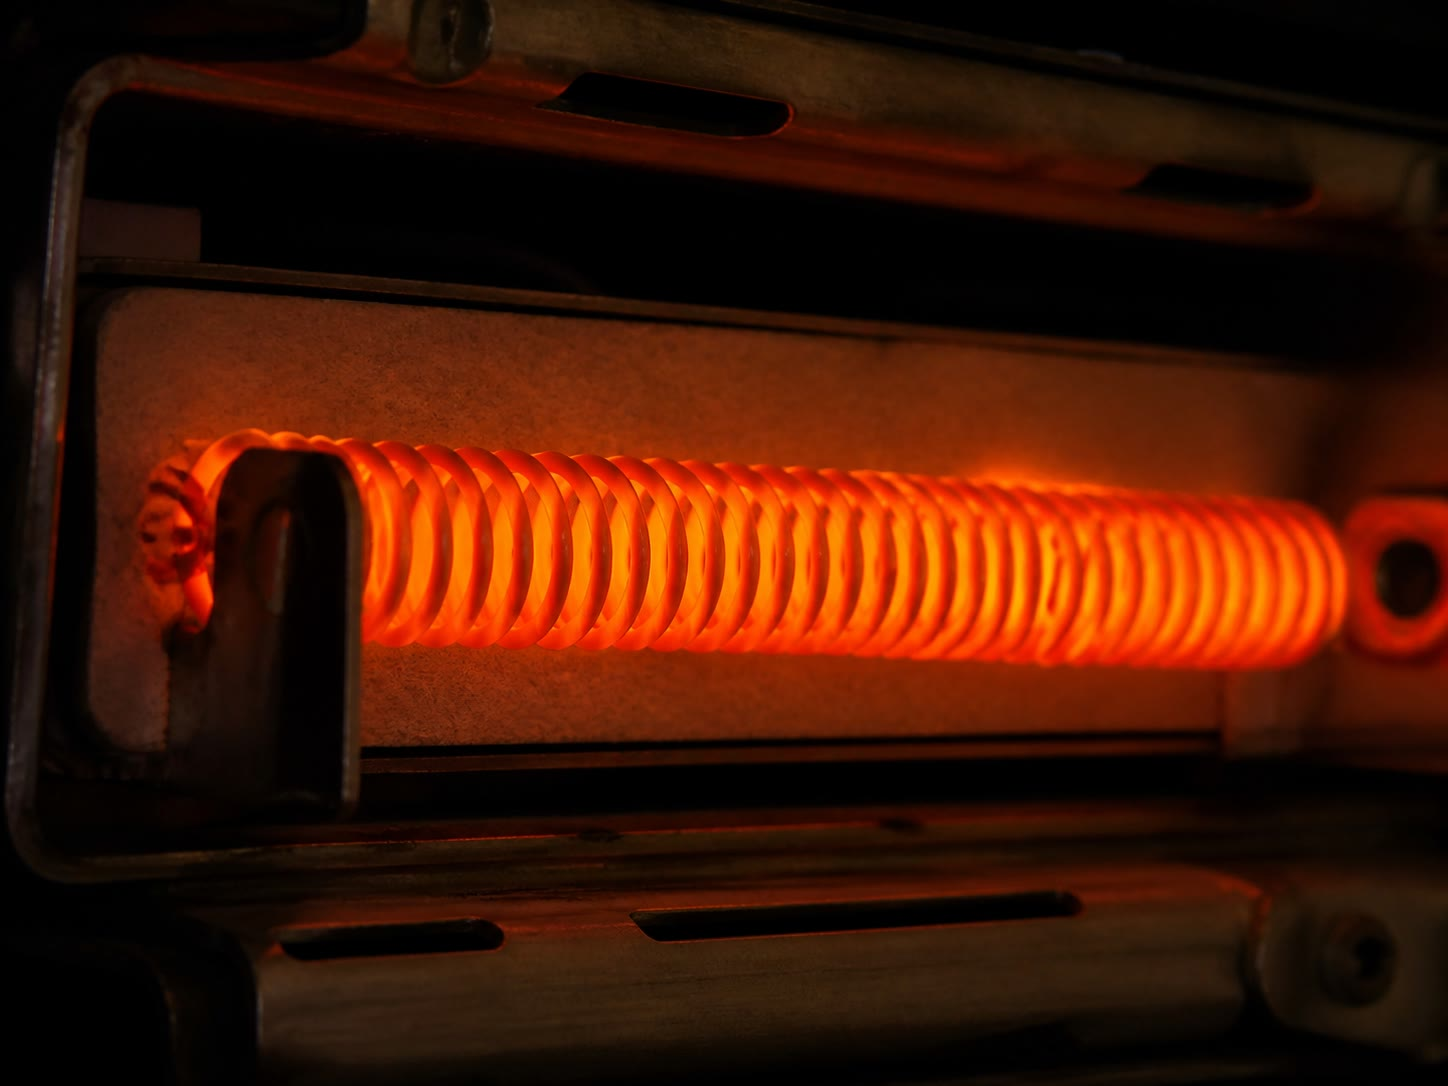
\includegraphics[width=0.5\linewidth]{images/book1/ai/g8-current-heating-coil.jpg}

{\small Efek termalnya, berpijar: arus yang dipaksa menembus kumparan berhambatan pada pemanggang rotinya memanaskannya sampai merah membara.}
\end{omfigure}

\section{Arus membuat magnet}

\begin{example}[Kompas mengkhianati kawatnya]\label{ex:g8:electric-current-effects:oersted}
Dua abad yang lalu, di tengah sebuah kuliah, seorang fisikawan
memperhatikan jarum \omterm{def:g4:magnets-and-compass:compass}{kompas} berkedut tiap kali ia menutup sebuah
rangkaian di atas meja di sampingnya. Kedutan itu --- yang tidak lebih
daripada gemetar sebuah jarum --- adalah jembatan pertama yang pernah
terlihat di antara kelistrikan dan kemagnetan, dua ilmu yang sampai
saat itu seterpisah cuaca dan musik. Baringkan sebuah \omterm{def:g4:magnets-and-compass:compass}{kompas} di
samping sepotong kawat lalu nyalakan: jarumnya berayun ke samping;
balikkan arusnya, dan ia berayun ke arah yang lain. Arusnya
menciptakan kemagnetan di sekeliling dirinya, dengan sebuah arah.
\end{example}

\begin{definition}[Elektromagnet]\label{def:g8:electric-current-effects:electromagnet}
Sebuah \emph{elektromagnet}\index{elektromagnet} adalah gulungan kawat
berisolasi --- sering dililitkan pada inti besi --- yang menjadi
\omterm{def:g1:magnets:magnet}{magnet} selagi arus mengalir menembusnya: \omterm{def:g4:magnets-and-compass:poles}{kutub utara}, \omterm{def:g4:magnets-and-compass:poles}{kutub selatan},
kekuatan menyambar besi, dan segalanya. Tidak seperti \omterm{def:g1:magnets:magnet}{magnet} batu mana
pun, ia menaati sebuah \omterm{ex:g3:first-electric-circuit:switch}{sakelar}: arus menyala, \omterm{def:g1:magnets:magnet}{magnet} menyala; arus
padam, \omterm{def:g1:magnets:magnet}{magnet} lenyap; arus dibalik, kutubnya bertukar.
\end{definition}

\begin{omfigure}
\begin{tikzpicture}[scale=0.85]
  \draw[thick, fill=omExo, fill opacity=0.3]
    (1.2,1.0) rectangle (5.4,1.9);
  \foreach \x in {1.5,2.1,...,5.1} {
    \draw[very thick, omDef] (\x,0.82) arc (200:340:0.35 and 0.5);
  }
  \draw[thick, omDef] (1.3,0.95) -- (0.4,0.4);
  \draw[thick, omDef] (5.3,0.95) -- (6.2,0.4);
  \node[below, font=\small] at (0.5,0.3) {menuju baterainya};
  \node[above, font=\small] at (3.3,2.05) {inti besi di dalam gulungan};
  \draw[thick] (7.4,1.05) ellipse (0.32 and 0.14);
  \draw[thick] (8.15,1.3) ellipse (0.32 and 0.14);
  \draw[thick] (7.5,1.6) ellipse (0.32 and 0.14);
  \node[right, font=\small] at (8.7,1.3)
    {klip kertas: tertahan selagi sakelar tertutup};
\end{tikzpicture}

{\small \omterm{def:g8:electric-current-effects:electromagnet}{Elektromagnetnya}: sebuah gulungan dan sebuah arus membuat
\omterm{def:g1:magnets:magnet}{magnet} yang dapat diciptakan, dimusnahkan, atau dibalik oleh \omterm{ex:g3:first-electric-circuit:switch}{sakelar}.}
\end{omfigure}

\begin{example}[Kemagnetan yang dapat disakelar menjalankan dunia]\label{ex:g8:electric-current-effects:uses}
Derek tempat rongsokan mencengkeram sebuah mobil dengan \omterm{def:g8:electric-current-effects:electromagnet}{elektromagnet}
lalu menjatuhkannya dengan membuka sebuah \omterm{ex:g3:first-electric-circuit:switch}{sakelar} --- cobalah itu
dengan \omterm{def:g1:magnets:magnet}{magnet} batu. Kunci pintu listrik, \omterm{def:g3:sound-around-us:sound}{bunyi} klak sebuah relai,
palu bel pintu (sebuah \omterm{def:g8:electric-current-effects:electromagnet}{elektromagnet} yang menyambarnya ke arah belnya,
memutus arusnya sendiri, lalu melenting kembali: kerincingan yang
dijadikan hukum), kepala pembaca telepon zaman dahulu, dan --- yang
teragung --- setiap \omterm{ex:g6:circuits-and-safety:motor}{motor} listrik: kemagnetan buatan arus yang
mendorong melawan \omterm{def:g1:magnets:magnet}{magnet}, ribuan kali tiap sekon. \omterm{prop:g8:electric-current-effects:three}{Efek magnet} adalah
otot zaman kelistrikan.
\end{example}

\begin{method}[Melilit sebuah elektromagnet]\label{met:g8:electric-current-effects:wind}
\begin{enumerate}
  \item lilitkan semeter atau dua \omterm{def:g2:measuring-length:units}{meter} kawat tipis berisolasi dalam
        lilitan yang rapat dan rapi mengelilingi sebatang paku besi
        atau baut yang besar, sambil menyisakan dua ujung yang bebas;
  \item hubungkan ujungnya ke sebuah \omterm{def:g3:first-electric-circuit:battery}{baterai} lewat sebuah \omterm{ex:g3:first-electric-circuit:switch}{sakelar}
        (jangan pernah langsung untuk waktu lama --- gulungannya
        hampir merupakan \omterm{def:g7:short-circuits-safety:device}{korsleting} lalu menghangat: efek panasnya
        mendampingi percobaannya);
  \item tutuplah \omterm{ex:g3:first-electric-circuit:switch}{sakelarnya} sejenak: kepala pakunya menyambar
        penjepit kertas; bukalah: penjepitnya jatuh;
  \item ujilah dengan sebuah \omterm{def:g4:magnets-and-compass:compass}{kompas}: kedua ujung gulungannya
        berperilaku sebagai kutub U dan S --- lalu bertukar ketika
        kamu membalik \omterm{def:g3:first-electric-circuit:battery}{baterainya}.
\end{enumerate}
Makin banyak lilitannya, makin kuat cengkeramannya: takarlah
kemagnetannya dengan melilit.
\end{method}

\section{Efek kimianya}

\begin{example}[Arus menembus air]\label{ex:g8:electric-current-effects:electrolysis}
Celupkan dua elektrode dari isi pensil yang terhubung kabel ke sebuah
\omterm{def:g3:first-electric-circuit:battery}{baterai} ke dalam air yang dibuat sedikit menghantar (sesendok soda
cuci membantu), lalu perhatikan: gelembung mungil mengalir dari kedua
isinya --- dua \omterm{def:g3:solids-liquids-gases:gas}{gas} yang berbeda, yang lahir dari airnya sendiri,
dengan \omterm{def:g6:mass-and-volume:volume}{volume} dua kali lipat pada isi yang satu dibandingkan yang
lain. Arusnya sedang membongkar air menjadi kedua penyusunnya yang tak
terlihat. Pintu di antara kelistrikan dan kimia ini ---
\emph{elektrolisis} --- menyepuh sendok murah dengan perak,
memenangkan aluminium dari bijihnya, dan sebagian besar menjadi milik
pelajaran kimiamu; fisika memberi hormat lalu berjalan terus.
\end{example}

\begin{example}[Setiap baterai adalah efek itu yang dijalankan terbalik]\label{ex:g8:electric-current-effects:battery}
Di dalam setiap \omterm{def:g3:first-electric-circuit:battery}{baterai}, kimialah yang mendorong arusnya: \omterm{def:g5:everyday-energy:energy}{energi} kimia
yang tersimpan menggerakkan arak-arakannya, sambil membelanjakan
dirinya selagi ia mengabdi --- pengosongan yang kamu kenal sejak
senter meredup. Sel yang dapat diisi ulang menutup lingkarannya:
pengisinya memaksa arus menembus \emph{terbalik}, dan \omterm{prop:g8:electric-current-effects:three}{efek kimianya}
membangun ulang simpanannya. Kimia menjadi listrik, listrik menjadi
kimia: satu efek, kedua arahnya, dan seluruh industri \omterm{def:g3:first-electric-circuit:battery}{baterai}.
\end{example}

\begin{remark}[Efek sebagai pengesan]\label{rem:g8:electric-current-effects:detect}
Ketiga efeknya menjawab sebuah pertanyaan yang membuatmu tertegun
ketika menjadi murid sang penguji: bagaimana kamu \emph{melihat}
sebuah arus --- arak-arakan tak terlihat di dalam kawat yang \omterm{def:g7:light-sources-propagation:coats}{buram}?
Lewat perbuatannya. Kawat yang menghangat, \omterm{def:g4:magnets-and-compass:compass}{kompas} yang berkedut,
gelembung yang mengalir: masing-masing mengkhianati arak-arakannya.
Setiap alat pengukur arus yang pernah dibangun membaca salah satu di
antara ketiga efeknya --- dan alat yang menanti pada bab berikutnya
membaca kedutan \omterm{def:g1:magnets:magnet}{magnetnya}, yang disempurnakan menjadi papan berangka.
\end{remark}

\section{Latihan}

\begin{exercise}[$\star$]\label{exo:g8:electric-current-effects:1}
Sebutkan ketiga efek \omterm{def:g7:circuits-series-parallel:current}{arus listrik}, masing-masing dengan satu kegunaan
yang mengabdi.
\end{exercise}

\begin{exercise}[$\star$]\label{exo:g8:electric-current-effects:2}
Efek yang mana, pada tiap adegan: \omterm{def:g7:short-circuits-safety:fuse}{sekring} yang melebur; \ bel pintu
yang memalu; \ gelembung pada isi pensilnya; \ nyala pemanggang roti;
\ cengkeraman derek tempat rongsokan?
\end{exercise}

\begin{exercise}[$\star$]\label{exo:g8:electric-current-effects:3}
Apa yang diungkapkan \omterm{def:g4:magnets-and-compass:compass}{kompas} yang berkedut di samping meja kuliah itu?
Apa yang terjadi pada kedutannya ketika arusnya dibalik?
\end{exercise}

\begin{exercise}[$\star$]\label{exo:g8:electric-current-effects:4}
Berikan tiga kekuatan yang dimiliki \omterm{def:g8:electric-current-effects:electromagnet}{elektromagnet} yang tidak dapat
ditandingi \omterm{def:g1:magnets:magnet}{magnet} batu mana pun.
\end{exercise}

\begin{exercise}[$\star$]\label{exo:g8:electric-current-effects:5}
Pada cara melilitnya, mengapa kawatnya harus berisolasi? Dan mengapa
gulungannya tidak boleh tetap terhubung lama tanpa beban yang bekerja?
\end{exercise}

\begin{exercise}[$\star$]\label{exo:g8:electric-current-effects:6}
Bagaimana juru dereknya melepaskan mobilnya? Bandingkan dengan apa
yang akan dituntut \omterm{def:g1:magnets:magnet}{magnet} batu yang sama kuatnya.
\end{exercise}

\begin{exercise}[$\star$]\label{exo:g8:electric-current-effects:7}
Perubahan \omterm{def:g5:everyday-energy:energy}{energi} apa yang terjadi di dalam sebuah \omterm{def:g3:first-electric-circuit:battery}{baterai} yang sedang
dipakai? Dan di dalam \omterm{def:g3:first-electric-circuit:battery}{baterai} isi ulang pada pengisinya?
\end{exercise}

\begin{exercise}[$\star$]\label{exo:g8:electric-current-effects:8}
Mengapa ketiga efeknya berharga sebagai \emph{pengesan}? Efek yang
mana yang akan disempurnakan alat bab berikutnya menjadi sebuah
bilangan?
\end{exercise}

\begin{exercise}[$\star\star$]\label{exo:g8:electric-current-effects:9}
Bel pintunya: sebuah \omterm{def:g8:electric-current-effects:electromagnet}{elektromagnet} menyambar palunya ke arah belnya,
tetapi palu yang bergerak itu memutus rangkaiannya sendiri; sebuah
pegas mengembalikannya, sehingga membuat ulang persentuhannya --- dan
seterusnya. Telusurilah satu daur penuh lalu jelaskan mengapa
rancangannya \emph{harus} berkerincing alih-alih menahan.
\end{exercise}

\begin{exercise}[$\star\star$]\label{exo:g8:electric-current-effects:10}
Sebuah relai adalah \omterm{ex:g3:first-electric-circuit:switch}{sakelar} yang ditutup oleh \omterm{def:g8:electric-current-effects:electromagnet}{elektromagnet}: arus
kecil di dalam gulungannya menutup persentuhan yang membawa arus besar
di dalam rangkaian yang lain. Jelaskan mengapa hal ini membiarkan
termostat yang halus memerintah pemanas listrik yang rakus dengan
aman --- dan kedua rangkaian mana yang tidak pernah bersentuhan.
\end{exercise}

\begin{exercise}[$\star\star$]\label{exo:g8:electric-current-effects:11}
Jarum kompasmu berkedut setiap kali sebuah kawat tersembunyi di dalam
dinding membawa arus. Rancanglah pencari kawat dinding dari kenyataan
ini: tata caranya, apa arti kedutan yang kuat, dan satu batas yang
jujur pada alatnya (pikirkan apa lagi yang menggerakkan jarum \omterm{def:g4:magnets-and-compass:compass}{kompas}).
\end{exercise}

\begin{exercise}[$\star\star\star$]\label{exo:g8:electric-current-effects:12}
Sebuah \omterm{ex:g6:circuits-and-safety:motor}{motor} listrik, secara garis besar: sebuah gulungan pada poros
duduk di antara kutub sebuah \omterm{def:g1:magnets:magnet}{magnet}; arus menjadikan gulungannya
\omterm{def:g1:magnets:magnet}{magnet}; dorong-dan-tarik kutubnya memutar porosnya --- dan tepat
ketika gulungannya hendak diam sejajar, arus yang menembusnya dibalik,
sehingga ia harus mengejar kesejajarannya selamanya. Jelaskan, kutub
demi kutub, mengapa pembalikannya tidak dapat ditinggalkan --- apa yang
akan dilakukan \omterm{ex:g6:circuits-and-safety:motor}{motornya} tanpa pembalikan itu? (Kamu baru saja
menjelaskan mengapa \omterm{ex:g6:circuits-and-safety:motor}{motor} memuat sebuah persentuhan pembalik --- dan
separuh dari cara zaman kelistrikan memutar rodanya.)
\end{exercise}

\section{Soal: Bengkel Sang Penemu}

\begin{problem}[{Soal akhir pekan --- satu baterai, tiga efek, lima
penemuan; sesore di bengkel sang
penemu}]\label{pb:g8:electric-current-effects:1}
Meja bengkelnya memuat \omterm{def:g3:first-electric-circuit:battery}{baterai}, kawat, paku besi, sebuah \omterm{def:g4:magnets-and-compass:compass}{kompas}, dua
isi pensil, sebuah toples air soda --- dan sebuah buku catatan berisi
penemuan setengah jadi yang harus dinilai.

\medskip\noindent\textbf{Bagian I --- Menghitung persediaan.}
\begin{enumerate}
  \item Sketsakan meja uji tiga efek milik bengkelnya: untuk satu
        \omterm{def:g3:first-electric-circuit:battery}{baterai} dan satu \omterm{ex:g3:first-electric-circuit:switch}{sakelar}, gambarkan susunan yang
        memperlihatkan ketiga efeknya sekaligus (sepotong kawat tipis
        untuk menghangat, sebuah \omterm{def:g4:magnets-and-compass:compass}{kompas} di samping sebuah isi pensil,
        toplesnya di dalam lingkarnya). Dalam susunan yang mana
        ketiga peragaannya harus duduk --- seri atau paralel --- supaya
        satu \omterm{ex:g3:first-electric-circuit:switch}{sakelar} menjalankan semuanya?
  \item Kawat peragaan yang tipis itu menghangat tetapi kawat
        penyalur yang tebal tetap sejuk, di dalam lingkar yang sama.
        Kenyataan mana dari bab satu tentang lingkar serinya yang
        membuat hal ini \emph{lebih} menarik daripada tampaknya ---
        apa yang sama pada kedua kawatnya, dan apa yang berbeda?
  \item Kompasnya berkedut ke timur ketika \omterm{ex:g3:first-electric-circuit:switch}{sakelarnya} tertutup. Dua
        perubahan apa, kalau dilakukan bersama, yang akan membiarkan
        kedutannya persis seperti semula?
  \item Gelembungnya mengalir dua kali lebih cepat dari isi pensil
        yang satu daripada yang lain. Apa yang diisyaratkan hal ini
        tentang kedua penyusun air? (Kimia akan menegaskan
        perbandingannya.)
\end{enumerate}

\medskip\noindent\textbf{Bagian II --- Menilai penemuannya.}
\begin{enumerate}[resume]
  \item Penemuan: ``bel pintu yang sunyi'' --- sebuah \omterm{def:g8:electric-current-effects:electromagnet}{elektromagnet}
        yang menarik palu kempa yang lembut sekali lalu menahannya
        sampai tombolnya dilepaskan. Bagian mana dari mekanisme bel
        pintu yang klasik yang harus \emph{disingkirkan} penemunya,
        dan apa yang akan didengar tamunya?
  \item Penemuan: ``pemilah \omterm{def:g1:magnets:magnet}{magnet}'' --- rongsokan di atas ban
        berjalan lewat di bawah sebuah \omterm{def:g8:electric-current-effects:electromagnet}{elektromagnet} yang mengangkat
        keluar besi dan baja. Apa yang terjadi di bak penjatuhannya,
        dan mengapa pemilahnya meninggalkan kaleng aluminium di atas
        sabuknya (dua kenyataan \omterm{def:g1:magnets:magnet}{magnet} dari tahun-tahun sebelumnya
        menjawabnya)?
  \item Penemuan: ``pembalik kutub'' --- sebuah \omterm{def:g4:magnets-and-compass:compass}{kompas} yang dipasang
        di atas sebuah gulungan, yang membalik tiap kali sebuah
        \omterm{ex:g3:first-electric-circuit:switch}{sakelar} tersembunyi membalik \omterm{def:g3:first-electric-circuit:battery}{baterainya}. Sifat kemagnetan
        buatan arus yang mana yang sedang dimanfaatkan?
  \item Penemuan: ``penyepuh abadi'' --- penyepuhan perak yang
        ditenagai \omterm{def:g3:first-electric-circuit:battery}{baterai} yang ``mengisi ulang dirinya sendiri dari
        penyepuhannya''. Tolaklah, sambil menyebut kedua arah \omterm{def:g3:first-electric-circuit:battery}{baterai}
        pada babnya dan sebuah hukum lama tentang \omterm{def:g5:everyday-energy:energy}{energi}.
\end{enumerate}

\medskip\noindent\textbf{Bagian III --- Adikarya malam itu.}
Penemunya menutup dengan sebuah permainan derek untuk pasar malam:
sebuah \omterm{def:g3:levers-and-scales:lever}{tuas} kendali, sebuah \omterm{def:g8:electric-current-effects:electromagnet}{elektromagnet} kecil pada tali, dan sebuah
bak berisi pernik besi.
\begin{enumerate}[resume]
  \item Tuliskan naskah gerakan yang menang dalam bahasa efeknya: apa
        yang terjadi ketika ``menyambar'', selama ayunannya, dan
        ketika ``melepaskan''?
  \item Pengunjung pasar mengeluh bahwa dereknya menjatuhkan hadiah
        di tengah ayunan setiap kali \omterm{def:g3:first-electric-circuit:battery}{baterai} tuanya melemah. Sifat
        \omterm{def:g8:electric-current-effects:electromagnet}{elektromagnet} yang mana --- keutamaan sekaligus kelemahan
        dalam satu --- yang sedang dipertontonkan?
  \item Penemunya menggandakan lilitan gulungannya untuk menolong.
        Ramalkan efeknya pada cengkeramannya, lalu sebutkan takaran
        yang satu lagi (dari sisi \omterm{def:g3:first-electric-circuit:battery}{baterainya}) yang akan dapat kita
        bilangkan pada bab berikutnya.
  \item Halaman terakhir buku catatannya: tulislah ringkasan
        bengkelnya --- satu kalimat tiap efek, masing-masing menyebut
        penemuan pengabdinya yang terbaik malam itu.
\end{enumerate}
\end{problem}
